% !TEX root = MasterThesis.tex

\chapter{Modern Operating System Concepts}\label{ch:modern-os-concepts}
%
%https://groups.google.com/forum/#!topic/comp.os.minix/wlhw16QWltI%5B1-25%5D
 % 2: your job is being a professor and researcher: That's one hell of a
% good excuse for some of the brain-damages of minix. I can only hope (and
% assume) that Amoeba doesn't suck like minix does.
% >1. MICROKERNEL VS MONOLITHIC SYSTEM
% True, linux is monolithic, and I agree that microkernels are nicer. With
% a less argumentative subject, I'd probably have agreed with most of what
% you said. From a theoretical (and aesthetical) standpoint linux looses.
% If the GNU kernel had been ready last spring, I'd not have bothered to
% even start my project: the fact is that it wasn't and still isn't. Linux
% wins heavily on points of being available now.
%
This thesis' introduction already picked up the discussion about which operating system architecture is the superior one by refering to the \textit{Tanenbaum-Torvalds debate}\cite{linux-is-obsolete} in 1992.
Besides the discussion is quite interessting from todays view on different operating systems, the forecasts on their future and the actual development, are both, \textsc{Tanenbaum} and \textsc{Torvalds} underpinning their arguments with the origins of their implementations \textit{MINIX} and \textit{Linux} in different problems. 
And roughly spoken are exactly such different problems which needs to be solved with an operating system one reason for their diversity. 
Over the years, they had to fit in solving very different kinds of problems on very different kinds of hardware, which resulted in many different ways of working and architectures. 
As with the debate, it is rather difficult to impossible to find one architectural concept or implementation which is clearly superior to the other ones in every use-case. 
Nevertheless, it is a reasonable question why a majority of the operating system kernels which were developed from scratch in the last few years are based on a microkernel concept.
In 2009, the official statement of the Linux kernel developer \textsc{Richard Gooch} was still that monolithic kernels are superior for performance reasons\cite{why-linux-monolith}.
So the question remains what changed during the last ten years to promote this change, and especially for this work, how this affects on device driver development.
For this reason, this chapter is dedicted to the basic components and functionallities of operating system kernels and how they are implemented in the real world examples \textit{Linux} and \textit{Zircon}.


%%%%%%%%%%%%%%%%%%%%%%%%%%%%%%%%%%%%%%%%%%%%%%%%%%%%%%%%%%%%%%%%%%%%%%%%
% Links
%
% Some notes to Linux design decisions: \url{http://vger.kernel.org/lkml/#s15-3}
% Memory management in Linux -> Files from LFD 430
% 
%
%%%%%%%%%%%%%%%%%%%%%%%%%%%%%%%%%%%%%%%%%%%%%%%%%%%%%%%%%%%%%%%%%%%%%%%%


\section{Operating System Architectures}\label{sec:kernel-arch-concepts}

% TODO OS design goals see Betriebssysteme Glatz 
As already pointed out are architectural decisions for operating systems commonly influenced by the issues they are intended to solve.
By giving priority to some design objectives that are pertinent to the underlying issue, different concepts and architectures are the outcome.
According to \textsc{Glatz}\cite{glatz2015betriebssysteme} are some of them:
\begin{itemize}
    \item Providing a reliable, crash-proof environment.
    \item Providing a portable operating system.
    \item Providing a scalable operating system, e.g.\ in terms of processing cores.
    \item Providing an extensibile operating system, e.g.\ in terms of adding additional functionality to the kernel.
    \item Providing real-time capabilities.
    \item Providing an efficient design in terms of ressources and performance.
    \item Providing a secure environment for user applications.
    \item Providing a maintainable operating system, e.g.\ by the division of policy and mechanism. 
\end{itemize}\ \\
%
In addition, operating systems should also pay attention to the common software design issue \textit{mechanism vs.\ policy}.
That means an operating system design should provide a clear distinction between the \textit{mechanism}, that means the capable abilities that can be performed (how is something done) and the \textit{policy}, which controlls how the available capabilities are used (what is done)\cite{lfd430},~\cite{silberschatz2009operating}.
An example for driver development could be controlling the number of processes that can use a device at once.
In this case, the driver should provide the mechansim, the \textit{how} such a limitation could be done, but not \textit{what}, the actual number of allowed processes. 
The idea behind is that requirements may change over some time and such a distinction makes it easy to adjust the \textit{policy} via some parameters without touching the underlying \textit{mechanism}\cite{silberschatz2009operating}.

How these design principles fit into the known operating system architectures will be considered in the following sections.
But before, the terms \textit{kernel mode} and \textit{user mode} will be explained as they are fundamental for this work.

\subsubsection*{Dual-Mode Execution}
Modern general purpose \acp{cpu} provide a ring based, hardware enabled security model which had it's origin in the Intel x86 processor architecture\cite{tanenbaum-modern-operating-systems}.
It is usually made of four different security levels, the rings 0 to 3 which are illustrated in Figure~\ref{pic:x86rings}.
In this model, ring 3 is the least secure level, used for common user applications (even if started with extended privileges (\textit{root} for the UNIX-like world)), while ring 2 is used for libraries shared between user applications and ring 1 is for system calls\cite{glatz2015betriebssysteme}.
System calls provide the transition to ring 0, the one with the topmost security level, which is used for the operating system kernel.
As a crucial part of an operating system, they will be discussed in more detail later in this work.

Directly related to this model is the \textit{dual-mode} execution mode of modern \acp{cpu}.
It is a hardware enabled security concept to provide a distinction between the user applications in ring 3 and the actual operating system kernel in ring 0.
Just the kernel in ring 0, running in the \textit{kernel mode} (or \textit{privileged mode, supervisor mode or system mode}), has direct and privileged access to memory, hardware, timers or interrupts, e.g.\ for performing \ac{io} operatings or memory mappings\cite{lfd430}.
User applications in ring 3, running in the \textit{user mode}, are not allowed to them so directly, they have limited privileges and a limited instruction set.
As named above, they need to use a mechanism called \textit{system calls} to transfer the execution to the \textit{kernel mode} where the priviledged actions are performed.
Lastly, the execution is transfered back to the calling user process and with this, the mode changes back to \textit{user mode}.
Figure~\ref{pic:mode-switches} pictures the operating flow of a system call including the mode switches between \textit{user} and \textit{kernel mode}.

%
%
\begin{figure} [ht]
	\centering
	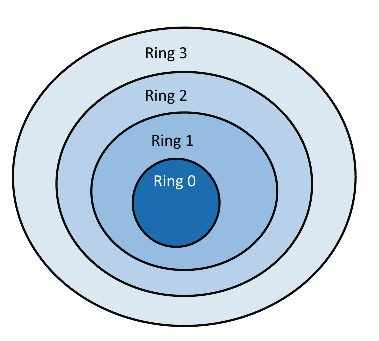
\includegraphics[scale=0.6]{x86Rings}
	\caption{The Rings of the x86's security concept\cite{glatz2015betriebssysteme}}\label{pic:x86rings}
    %TODO own picture!
\end{figure}
%
\begin{figure} [ht]
	\centering
	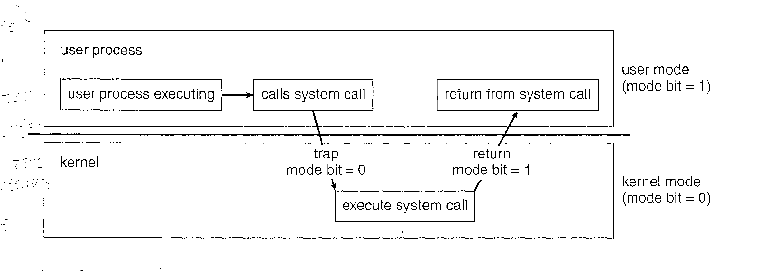
\includegraphics[scale=0.6]{mode-switch}
    \caption{A system calls sequence including the mode switches\cite{glatz2015betriebssysteme}}\label{pic:mode-switches}
    %TODO own picture!
\end{figure}

The \ac{cpu}'s operating mode is usually controlled by a specific bit in the \ac{psw}\cite{tanenbaum-modern-operating-systems}.
It influences the state of each \ac{cpu} core itself in a multi-processor system, but not the operating system kernel.
As a result, different \ac{cpu} cores may be in a different execution mode\cite{lfd430}.
With this seperation, any priviledged instruction is forbidden in \textit{user mode} and will not be executed.

Based on the dual mode execution on the \ac{cpu}, different architectural concepts for operating systems evolved.
They differ e.g.\ in the share of the operating system respectively the operating system's kernel actually running within the \ac{cpu}'s \textit{kernel mode}. 
Thus, they have an influence on the whole system, including device driver development but also on performance and security issues.

With this basic knowledge about the \ac{cpu}'s operating modes, the next section researches a selection of different operating system architectures.
Special attention should be paid to the most common ones, the \textit{monolithic} and the \textit{microkernel} architectures and their implementation in Linux and Zircon.
On the contrary, this work will not take a particular look on special purpose operating system architectures such as ones for loosely coupled multi-processor systems known from processing clusters.
Today, even the majority of general purpose computing systems are driven by more than one \ac{cpu} and most of common modern operating systems are designed to provide support for the defacto standard for tightly coupled systems, \ac{smp}.


\subsection{Monolithic Architectures}\label{sec:monolithic-archs}
Some sources, such as \textsc{Glatz}\cite{glatz2015betriebssysteme} or \textsc{Silberschatz}\cite{silberschatz2009operating}, suggest monolithic operating systems do not have a well-defined structure at all. 
As they are indeed most commonly grown structures, started in a completely different scope (MS-DOS, the original UNIX), it is not an incorrect claim.
But it does not neccessarily have to be the case.
Above all, monolithic operating system (kernel) architectures have in common that they form one single binary program which is running entirely in kernel mode.
User programms, running in user mode, interact with the kernel only through a well defined set of \textit{system calls}\cite{lfd430}. 
Within the kernel itself, all parts are free to use and access each other but also the hardware, without any limitation, e.g.\ regarging the access of kernel functionalities of another component or hardware acces. 
That means a function or procedure initial developed for scheduling processes could be used in a completely different context if its functionality is useful to solve another issue.
In fact, there is no information hiding between kernel functions or procedures.
Any function in this kernel context has full access to the hardware, such as \ac{io} devices, timers, interrupts and even to the memory. 
There is no memory protection or validation between different components of a monolithic kernel. 
Of course, this leads to some serious disadvantages in this architecture, for example could a crash in one single function or procedure crash the entire kernel or the resulting system may become difficult to understand and maintain\cite{tanenbaum-modern-operating-systems},~\cite{silberschatz2009operating}.
The missing memory protecting within the kernel could also be a source for crashes or attacks.
But in contrast, this design also enables a very efficient kernel design without any unneeded communication overhead or hardware inefficiencies\cite{lfd430}.

An extension of the monolithic architecture are the so-called \textbf{modular operating systems}.
They provide additional, defined interfaces for (in common) dynamically loadable and unloadable extentions, e.g.\ for device drivers or filesystems. 
Sometimes, such extensions or modules are just allowed to use a limited function set of the operating system, but they are still running as a part of the kernel in kernel mode\cite{lfd430},~\cite{tanenbaum-modern-operating-systems}. 
Just like ordinary kernel functions or procedures, (malicious) programming errors in extentions may lead to a kernel crash or manipulate or damage other components.
Contrary, the modular concept provides some advantages over regular monolitic kernels.
It allows to slim down the actual kernel by providing the chance to reload only the actually needed functionality dynamically and e.g.\ security patches within such an extension is possible without restarting the entire system\cite{brause2017betriebssysteme}.
As the extensions become an part of the operating system running in kernel mode, no additional communication effort between the actual kernel and the modules is required.
Thus, concept of modules is quite popular for basically monolithic operating systems like \textit{Linux} or \textit{Solaris}\cite{brause2017betriebssysteme},~\cite{silberschatz2009operating}.


\subsection{Microkernel Architectures}\label{sec:microkernel-archs}
The microkernel architecture focuses on very opposite design goals compared to the monolithic one. 
Some of them are to cope the complexity, rather poor maintainablity and susceptibility to errors by a massively modular approach. 
To archive this, the core idea behind microkernels is to provide only a very small kernel running in kernel mode which only provides the core functionalities while all the other important functions of an operating system are running in user mode.
Thereby, the microkernel architecture is excellently suited to implement a proper division of mechanism and policy.
The kernel provides just the most basic mechanisms needed for an operating system, while the userspace modules implement the policy.
This decoupling makes it easier to change the policy in userspace for altering requirements without touching the actual kernel\cite{tanenbaum-modern-operating-systems}.

What is part of this core functionality differs between miscellaneous sources, but all considered ones are in agreement that a simple mechanism for process scheduling is as well a core functionality as providing an \ac{ipc} mechanism\cite{lfd430},~\cite{silberschatz2009operating},~\cite{glatz2015betriebssysteme}.  
In contrast, the sources disagree as to whether memory management and virtualisation, device drivers or synchronization facilities are a part of the actual kernel.
The \textit{Mach} microkernel, which formed the first generation of microkernels in 1985, named process and thread administration, an extensible and secure \ac{ipc} mechanism, virtual memory management and scheduling as its core tasks, while everything else needed has to run in usermode\cite{rashidMach}.
Functional enhancements of the system do not require changes to the kernel itself, too.
This concerns, depending on the exact relization, device drivers, memory management, system call handlers and even more system components\cite{lfd430},~\cite{silberschatz2009operating}.
In academic microkernel approaches, all components in user mode run within an own userspace process as small, well-defined modules, while the communication is done through copious message passing via the actual kernel\cite{tanenbaum-modern-operating-systems},~\cite{lfd430}.
Since the restrictions by the \ac{cpu}'s dual mode still apply for microkernel based operating systems is it not allowed to device drivers running in user mode to have direct physical access to \ac{io} ports as a consequence.
A device driver has to invoke the actual kernel to perform the needed action substitional.
But thus, the kernel is able to check the action and whether the driver is authorized to executed them.
Resulting, the microkernel design is more reliable and secure as such a division enables the kernel to intercept erroneous actions such as accidental memory writes to important regions\cite{tanenbaum-modern-operating-systems}.
Equally a crash in a userspace system component like a driver is not able to crash the entire kernel in such an approach. 
And as an additional advantage facilitate the microkernel architecture porting the operating system kernel to another target architecture as the most hardware dependencies are part of the small kernel\cite{silberschatz2009operating},~\cite{lfd430}.

With all the named advantages microkernels offer, the question remains why microkernels are only spread in real-time, avionics or military but not for desktop operating systems.
One reason is that all these advantages are bought at the high price of microkernel message costs.
For the named application areas, especially the reliability that comes with the microkernel architecture is more desirable than the performance costs of the lot more context switches in comparison to monolithic architectures\cite{tanenbaum-modern-operating-systems}.
Since a lot of the operating system's functionality has been moved to the userspace, microkernel architectures need to perform noticable more context switches to invoke the actual kernel for privileged actions. 
The performance losses are not only caused by the large amount of context switches themselves, but also by the fact that modern \acp{cpu}, particularly the caches are not designed for them. 
Every context switch causes cache misses which trigger that the required data has to be loaded from the slower main memory and cached. 
The data of the previous context (e.g.\ the user mode context) will be displaced from the cache and the \ac{cpu} is largely blocked in the meantime.
By rapidly switching back to the previous context, as is usual for e.g.\ a short kernel invokation to perform an \ac{io} operation on microkernel architectures, the cache is no longer suitable for the new context and has to be replaced\cite{lfd430}.

First of all, the \textit{L4} kernel, a second generation microkernel was able to get close to the performance of a monolithic kernel as \textit{Linux} it is\cite{Hrtig1997}.   
Nevertheless are pure microkernels mainly used for systems with high reliability requirements but unusual for desktop application. 
Some industry examples are \textit{Integrity}, \textit{QNX} and \textit{seL4}, a mathematically verified version of the \textit{L4} kernel\cite{tanenbaum-modern-operating-systems}. 

%TODO ? reincarnation server : check if all modules are up running and work correctly -> if not it replaces them without user interaction \cite{tanenbaum}
%TODO picture \cite{microkernels}


\subsection{Layered Architectures}
Layered operating system architectures are usually organized in hierachical layers, but sometimes the choosen model is described as a series of concentric rings.
Each layer or ring provides a group of functionality while a it is only allowed to use the functions of the one directly below. 
The cooperating between the layers or rings is regulated by clearly defined interfaces\cite{brause2017betriebssysteme}.
This is usually accompanied by the fact that the lower layers or inner rings are more privileged as the outer ones.
However, there is no uniform and univerally accepted approach for division in layers and their count accoring to this pattern\cite{glatz2015betriebssysteme},~\cite{tanenbaum-modern-operating-systems}.
In fact, a meaningful division is not that easy.
Functionalities may have to be divided artifically and the harmonious arrangement can have its pitfalls caused by the access requirements this architecture is based on.
Is the layered access model considered properly to get a clean architecture, it that can unfold its advantages.
These are for example the interchangeability of the layers if they and their interfaces were properly designed or the resulting concept for debugging.
As the layers are constructed on top of each other, it is possible to debug  and verify each one for its own, starting at the lowest layer up to the top most one\cite{silberschatz2009operating}.
But also the costs for system calls are comparatively high, because they have to be passed though all layers while each one adds overhead to such a call\cite{silberschatz2009operating}.  

In general, layered operating system architectures are related to monolitic ones, but it is conceivable to adopt the idea for microkernel approaches, e.g.\ is the MINIX userspace divided into layers. 
Examples for this architecture are \textit{OS/2} or newer \textit{Unix} variants, while \textit{Multics} is one for a concentric rings based model\cite{glatz2015betriebssysteme},~\cite{tanenbaum-modern-operating-systems}.


% \subsection{Distributed Architectures}


\subsection{Hybrid Architectures}
Hybrid operating system architectures based on monolithic, microkernels and may be the layered ones are common approach to combine the advantages of these concepts.
They try to pair the performance of the monolithic design with the modularity and reliability of microkernels\cite{microkernels},~\cite{silberschatz2009operating}.
How both worlds interact is very different depending on the exact implementation.
\textsc{Silberschatz} explains one of them in his book \textit{Operating System Concepts}\cite{silberschatz2009operating} using Apple's \textit{OS X} (today named \textit{macOS}) as an example.
Depending on the exact implementation and the share of the architectures, most disadvantages of monolithic architectures still apply for the hybrid systems.
Further examples for hybrid architectures are \textit{Windows NT} and \textit{BeOS}\cite{microkernels}.  


\subsection{The Linux Kernel's Monolithic Architecture}

Linux is the perfect example for an extremly grown operating system.
Starting as a pure hobby project to learn about a specific \ac{cpu} and connect to the Unix computers at \textsc{Linus Torvalds}, its initial author's, university, it becomes strongly related to its archetype, \textit{Unix}\cite{DiamondTorvalds2002}. 
They share fundamental design goals, just like beeing capable of multiple processors and user at the same time, but Linux is not based on the origin Unix source code\cite{tanenbaum-modern-operating-systems}.
The overall architecture of the Linux kernel is, as already named, monolithic and also inspired by Unix\cite{lfd430},~\cite{DiamondTorvalds2002}.
It is entirely running in kernel mode and all built-in layers have full access to the internal kernel \ac{api} using common function calls like in C.
A sophisticated concept of kernel modules which can be dynamically loaded to a running kernel makes a limited number of microkernel advantages available for Linux.
Modules in Linux are only allowed to use a restricted (exported) set of functions to use, but once loaded to the running kernel, they become a part of the monolith running in kernel mode\cite{lfd430}.
Linux is largely compatible to the \ac{posix} standard which was initially created for Unix.
Initally, it was because \textsc{Torvalds} could not get a version of the standard, while today it is rather a conscious decision\cite{DiamondTorvalds2002},~\cite{tanenbaum-modern-operating-systems}. 
Also the decision for the monolithic architecture is today consciously supported by the kernel community and justified with its performance and efficiency over microkernels due to the \textit{priviledge barrier} between user and kernel mode which has to be passed quite often in microkernel architecture\cite{why-linux-monolith},~\cite{lfd430}.
The Linux kernel itself is divided in five essential tasks which are also reflected in its source code.
They are: 
\begin{itemize}
    \item Process Management,
    \item Memory Management,
    \item Filesystems,
    \item Device Management and
    \item Networking\cite{lfd430}.
\end{itemize}
By structuring this tasks and further components into \textit{subsystems} like \textit{drivers/}, \textit{fs/} (filesystems), \textit{net/} or \textit{kernel/}, the linux kernel remains comprehensible and in some ways modular. 
A closer look to the most of them in general but also their implementation in Linux is done in the following sections.

The Linux kernel is mainly written in C but some very hardware dependent part are in Assembly. 
Additionally, especially the Assembly parts were strongly dependent on the \ac{gcc}.
Today, there are some efforts to reduce the share of Assembly for maintenance and readability since modern compilers do not generate less efficient code as hand-written Assembly is\cite{programming-religion}.
This also reduces the dependency to \ac{gcc} and enables the use of alternative compilers, especially Clang\cite{linux-clang},~\cite{fosdem-linux-llvm}.
Nevertheless, the Linux kernel's principal lanugage is C and it only provides support for C drivers. 


\subsection{The Zircon Kernel's Microkernel Architecture}
% design goals, architecture, interface posix, parts, language/compiler
In contrast to the Linux kernel, Zircon is not a grown structure.
Started in 2015, it was largely developed from scratch by Google for a so far undisclosed field of application\cite{chat-zircon-arch}.
Nevertheless, Zircon emerged from a branch of \textit{Little Kernel} (LK) by \textsc{Travis Geiselbrecht} which is also a part of the Zircon Team at Google\cite{zircon-vs-lk}. 
Despite its origin, Zircon is very differnt to Little Kernel.
It targets powerful devices such as modern computers and phones and provides for this reason only 64-bit support, first class user-mode support and a capability-based security model. 
In contrast, Little Kernel is designed for embedded applications and amongst others used as bootloader for \textit{Android} and as \textit{Android Trusted Execution Environment (Trusty TEE)}\cite{lk-intro}.
It has 32-bit support, but none of the more sophisticated features Zircon has\cite{zircon-vs-lk}.

The mirokernel architecture is justified by having security, safety, reliability and modularity as major design goals for Zircon.
According to \textsc{Travis Geiselbrecht} was the architecture a conscious tradeoff between the named goals and performance\cite{chat-zircon-arch}.
They try avoid costly context switches as much as possible, speed up the remaining ones and take advantage from \ac{smp}, but it is not the focus of Zircon.
Alike, Zircon does not focus on performing \ac{io} operatings or process management which are the key tasks \ac{posix} was designed for\cite{chat-zircon-arch}.
As a result, Zircon does not claim to be or to become \ac{posix} compatible, they just support a very basic subset of the standard\cite{zircon-libc-posix}.
% For \ac{ipc} Zircon provides a mechansim based on an \ac{idl} which is widly used within the Zircon kernel but also in Fuchsia as the whole operating system.
The Zircon kernel itself is splitted up into the actual microkernel running in kernel mode (\textit{kernel/}) and services, drivers and core libraries running in user mode (\textit{system/})\cite{zircon-intro}.
The kernel part provides the basic operating system mechanisms: 
\begin{itemize}
    \item Process Management,
    \item (virtual) Memory Management,
    \item \acl{ipc} and
    \item Synchronization Mechanisms\cite{zircon-intro}.
\end{itemize}
The part running in user mode contains core services for, amongst others, booting, device management and networking, device drivers respectively hardware related code and user libraries.

Zircon is for the most parts written in C++ and less in C.
It provides native support for device drivers in both languages but due to the fact Zircon provides an \ac{idl} which defines a contract for in-process drivers, other languages are conceivable as well.
In fact, support for Rust drivers is currently beeing worked on\cite{chat-zircon-arch}.
Unlike Linux, Zircon provided support for both, the \ac{gcc} and the Clang compiler, from the beginning caused by the sophisticated tools aroung Clang and LLVM\@.


\section{System Calls}\label{sec:system-calls}
System calls were already marginally mentioned in this work as the mechanism to switch the program execution between user and kernel mode, because  applications running in user mode have only restricted rights.
Thus, this special calls are needed for the interaction with basic hardware devices like the \ac{cpu}, the memory, peripherals or filesystems and for invoke the actual operating system's kernel for management operations like process management\cite{lfd430}. 
System calls are to a high degree hardware dependent and differ between various operating system implementations.
% Even operating systems which comply the \acf{posix} standard may differ in the typ and number of available system calls.
% The wide-spread \ac{posix} standard is only an \ac{api} definition but not one for system calls.
% An operating system may implement the \ac{posix} standard functions within a library which often involve system calls, but it has not to do so\cite{lfd430},~\cite{glatz2015betriebssysteme}.
% Equally, a system is not constrained to a single \ac{api} and may implement different ones using its existing set of system calls\cite{glatz2015betriebssysteme}.
% \ac{posix} is implemented is a very common standard which is for example implemented in UNIX, macOS, MACH and partly in Linux\cite{tanenbaum-modern-operating-systems},~\cite{glatz2015betriebssysteme}.
% Another example for an \ac{api} is Win32 used by Windows to abstract their system calls.
% As a result system calls are rarely used directly by user applications without an abstraction layer such as libraries. An example is the \textit{libc}\cite{lfd430},~\cite{tanenbaum-modern-operating-systems}.
%

A system call has its origin in an application running in user mode.
If the application has to invoke the operating system kernel, e.g.\ to perform an action on memory in substition, it has to use one for switching the operating mode\cite{glatz2015betriebssysteme},~\cite{tanenbaum-modern-operating-systems}.
As switching the \ac{cpu}'s execution mode also means a new context, a system call to the kernel differs from a common procedure call.
In user mode, the so-called entry code stores the system call's parameters in a defined way.
One is to store the parameters and the call's number in defined registers (see~\ref{pic:syscalls}), another one is to store them on stack, according the C/C++ calling in reverse order\cite{silberschatz2009operating},~\cite{glatz2015betriebssysteme}.
The exact one depends on the actual \ac{cpu} architecture.
The following instruction triggers a specical software interrupt containing the order to switch the context.
It is also named \textit{trap instruction}\cite{glatz2015betriebssysteme},~\cite{tanenbaum-modern-operating-systems}.
To be exact, it is the interrupt vector number of the trap instruction which is responsible for the switch.
They are \texttt{0\x80} on Linux as pictured in~\ref{pic:syscalls} and \texttt{0\x2e} on Windows systems\cite{glatz2015betriebssysteme}.
But right before switching it is needed to save the \acf{psw}, which contains the actual processors state includes the mode bit, to the stack.
The same number is used in kernel mode as an index within the interrupt vector table (or interrupt discriptor table, IDT) which contains the start address of the system service dispatcher routine (compare to~\ref{pic:syscalls}).
This tables content, the system serice dispatcher routine, is loaded as next instruction to the new \ac{psw}\cite{brause2017betriebssysteme}.
Jumping to this routine, the system call's parameters and its number are restored to examine the actual call and invoke the matching service routine from the system service dispatching table which finally fulfils the requested action as simplified pictured in~\ref{pic:syscalls}\cite{glatz2015betriebssysteme}.
Conclusively, the control flow jumped back to the system service dispatcher which hands the controll back to user space inclunding switching back to user mode in the common way to return\cite{glatz2015betriebssysteme}.
The previous \ac{psw} is restored from stack containing the bit for \ac{cpu}'s user mode execution.
The user application has to clean up the stack like for each procedure call at the very end\cite{tanenbaum-modern-operating-systems}.

Figure~\ref{pic:syscalls} shows a simplified version of the system call implementation on x86 for Linux kernel before 2.5\cite{decade-linux-syscalls}.
More modern versions use the special instructions \texttt{SYSENTER} and \texttt{SYSEXIT} (Intel) or \texttt{SYSCALL} and \texttt{SYSRET} (AMD) instead of the slower trap interrupts\cite{decade-linux-syscalls}.

\begin{figure} [ht]
	\centering
	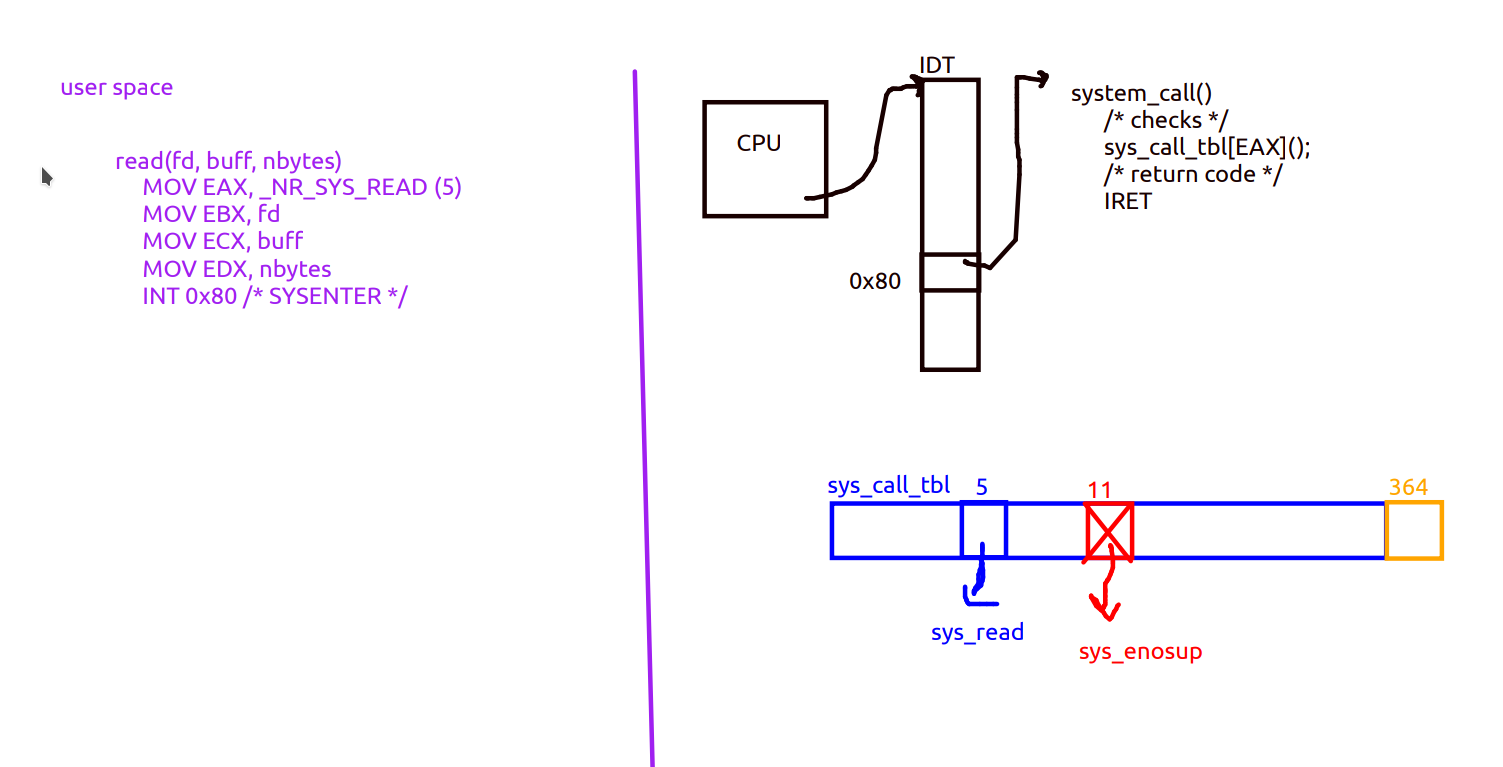
\includegraphics[scale=0.4]{syscall-lfd}
    \caption{System Call Implementation\label{pic:syscalls}\cite{lfd430}}
    %TODO own picture!
    %TODO add numbers and a kind of flow sequence with numbers. Add numbers to text.
\end{figure}


\subsubsection{POSIX}
The basic idea behind the \acf{posix} standard is to define a stable interface between the user-space and the operating system kernel to archieve portability for applications on systems meeting this standard.
But even if an operating system comply the them, it may differ in the typ and number of available system calls.
\ac{posix} is only an \ac{api} definition but not one for system calls.
An operating system may implement the \ac{posix} standard functions within a library which often involve system calls, but it has not to do so\cite{lfd430},~\cite{glatz2015betriebssysteme}.
System calls are rarely used directly by user applications without an abstraction layer such as libraries. An example is the \textit{libc} on Unix-like systems\cite{lfd430},~\cite{tanenbaum-modern-operating-systems}.
Equally, a system is not constrained to a single \ac{api} and may implement different ones using its existing set of system calls\cite{glatz2015betriebssysteme}.

\ac{posix} is a very common standard which is for example implemented in UNIX, macOS, MACH and partly in Linux\cite{tanenbaum-modern-operating-systems},~\cite{glatz2015betriebssysteme}. 
Another example for an \ac{api} is Win32 used by Windows to abstract their system calls, but as a result, applications targeting the Windows Win32 \ac{api} are not portable to systems implementing the \ac{posix} standard.
% As a result system calls are rarely used directly by user applications without an abstraction layer such as libraries. An example is the \textit{libc}\cite{lfd430},~\cite{tanenbaum-modern-operating-systems}.


\subsection{System Calls in Linux}
In fact, the way system calls are working in Linux was already described as part of the general section. 
The exact mechanism, the calling convention but also the number of system calls is highly depending on the \ac{cpu}'s architecture.
While a 32-bit Linux kernel in version 4.8 for the x86 architecture offered 379 calls, the 64-bit version for x86\_64 just offered 328\cite{lfd430}.
The \textit{man-pages} project documents gives an overview (\texttt{man 2 syscall}) about architectural differences and the calling conventions.
How far Linux is acutally compatible to the \ac{posix} standard is not only related to the kernel and the number of system calls itself, but for the most part to its abstraction layer, the used \ac{posix}/C standard library.
One of the most spread ones, the \textit{glibc} (GNU C Library) aims to follow POSIX.1\-2008 amoungst other standards\footnote{\url{https://www.gnu.org/software/libc/}} while the \textit{musl} library does not implement it in complete\footnote{\url{https://repo.or.cz/w/musl-tools.git/blob_plain/HEAD:/tab_posix.html}}.



\subsection{System Calls in Zircon}
% FIDL, core libs,.. 
% http://research.cs.queensu.ca/~cordy/Papers/BKBHDC_ESE_Linux.pdf
% for vdso
In Zircon, system calls are bounded to the concept of \textit{handles}, a construct allowing applications running in user mode to reference a object in kernel mode\cite{zircon-handle}.
Interactions between user applications and kernel objects are still done using system calls but the most of them are using a handle which describes the kernel object to work on\cite{zircon-concepts}. 
Handles are checked by the kernel each time a system call is triggered.
For additional security, the kernel checks wether
\begin{itemize}
    \item a handle has the correct type for the system call, 
    \item a kernel handles parameters refer to one existing within the calling process's handle table and
    \item a handle has the necessary rights for the triggered action\cite{zircon-concepts}.
\end{itemize}

In contrast to Linux, Zircon provides just one libary for system calls and the standard C implementation, the \textit{libzircon.so}.
It is a \acf{vdso} directly provided by the kernel and not stored as a physical ELF file on disk.
For the reason that \acp{vdso} are accessable from both, kernel and user mode, without switching the context, they are a perfect concept to implement system calls in a very performant way\cite{vdso-linuxjournal}.
Thus, the Zircon \ac{vdso} is the only way to perform system calls\cite{zircon-vdso}, which is a very elegant solution to cope with performance issues in a microkernel architecture.

The system calls are defined by using a abstract definition syntax and the matching tool \textit{abigen} which generates header files and code for the libzircon and the kernels system call implementation\cite{zircon-concepts}.
Also in contrast to Linux does Zircon respectively Fuchsia not aim for \ac{posix} compatibility.
It implements only a very limited subset of \ac{posix} consisting of basix \ac{io} operations and pthreads.
Zircon does not support Unix-like signals, symbolic links and much more\cite{zircon-libc-posix}.
The libzircon.so does not support directly \ac{io} operations. 
They are performed by the \textit{fdio.so} library which overwrites weak symbols of the libzircon\cite{zircon-libc-posix}.

\section{Processes and Threads} %TODO label
\subsection{Processes}
\subsection{Threads}
\subsection{Inter Process Communication}
\subsection{Scheduling}
\subsection{Processes and Threads in Linux}
\subsection{Processes and Threads in Zircon}


\section{Memory Management} %TODO label
%    Linux Concept -> LFD430 pic
%TODO find sections
%TODO how is it done in Linux and Zircon
\subsection{Address Spaces}
\subsection{Virtual Memory}
\subsection{Page Replacement/Paging}
\subsection{Memory Management in Linux}
\subsection{Memory Management in Zircon}


\section{I/O} %TODO label
%TODO review sections, how is it done in Linux/Zircon
\subsection{I/O Hardware}
\subsection{Memory Mapped IO}
\subsection{Direct Memory Access}
\subsection{Interrupts}
\subsection{Power Management}

   
\section{Security Concepts} %TODO label
\subsection{Access Control} %Domains, Capabilities
%DAC, MAC, ..
\subsection{Security Concepts in Linux}
\subsection{Security Concepts in Zircon}


\section{Driver Models} %TODO label
